\subsection{A3 School Leadership}
The school leadership (1) makes decisions to facilitate actions that focus the energies of the school on student achievement of the schoolwide learner outcomes, i.e., global competencies, (2) empowers the staff, and (3) encourages commitment, participation, and shared accountability for student learning in a global environment.

\subsubsection{Defined Responsibilities, Practices, etc.}

\indicator{The school has administrator and faculty written policies, charts, and handbooks that define responsibilities, operational practices, decision-making processes, and relationships of leadership and staff.}

\prompt{Evaluate these administrator and faculty written policies, charts, and handbooks. Determine the clarity and understanding of these by administration and faculty.}

\begin{findings}
CMIS has clear policies that define responsibilities, operational practices, decision making processes and relationships of leadership and staff. 

These policies and procedures can be found in the CMIS employment contracts and the \href{https://drive.google.com/a/cmis.ac.th/file/d/0ByVFfrm0zfolVm9uc19UNl82NVpPMUZ1ZEstZlFidEY1c2hn/view?usp=sharing}{CMIS Faculty Handbook}. They are reviewed annually during the administrative, new teacher, and returning staff orientations. 

Furthermore, a list of administrative teams is included in the Faculty Handbook and CMIS Student Planner. 

CMIS organized ``\href{https://drive.google.com/a/cmis.ac.th/file/d/0ByVFfrm0zfolbHNvSWhVWmJYU3M/view?usp=sharing}{Teacher Table Talk}'' sessions during early release days to capture insights and suggestions about the decision-making processes and relationships of leadership and staff. 

In November, 2016 the \href{https://docs.google.com/a/cmis.ac.th/document/d/1iW_tWIwRlWU2p0oIOvd3usDsxj9qYDt_2ROwNPBTHSc/edit?usp=sharing}{Teacher Leadership Team}  which is made up of teachers and administrators, participated in the revision of the handbook format and made it available in an electronic formatted version. We plan to make this an annual project as it was previously revised only by administrators.

CMIS Board governance requires the Executive Team (i.e. Superintendent, Director and Manager) to maintain up-to-date operational handbooks and procedural guidelines.

Board member roles and responsibilities are clearly outlined and described in the \textit{Christian Churches of Thailand Board Handbook}.

\minor{So what...}

CMIS Leadership has clearly defined roles for teachers only through a variety of methods, most notably the Teacher Handbook. CMIS should continue to maintain, monitor, and modify, as necessary, the Teacher Handbook with stakeholder feedback and input. Additionally, CMIS should develop a Leadership Handbook to clearly outline the roles and responsibilities of principals, directors, and team leaders.
\end{findings}

\subsubsection{Existing Structures}

\indicator{The school has existing structures for internal communication, planning, and conflict resolution.}

\prompt{How effective are the existing structures for internal communication, planning, and conflict resolution?}

\begin{findings}

CMIS has many existing structures for internal communication, planning, and resolving differences.

Communication and Planning Examples:
The School Executive Team (SET) shares information from the monthly Board of Director Meetings to the School Management Team (SMT), and to the \href{https://docs.google.com/a/cmis.ac.th/document/d/1iW_tWIwRlWU2p0oIOvd3usDsxj9qYDt_2ROwNPBTHSc/edit?usp=sharing}{Teacher Team Leaders} who communicate the information to the teachers.

Internal communication is also highlighted through Weekly \href{https://docs.google.com/a/cmis.ac.th/document/d/1Jh_VpJ8rfb4_OwmpRw6VZCrIYAuV6A0SP_3NN82KD7A/edit?usp=sharing}{HS Principal Notes}, \href{https://mail.google.com/mail/u/0/#search/tstinchcomb\%40cmis.ac.th/15a1132a902382f6?projector=1}{MS Principal Message THIS LINK IS BAD} and \href{https://mail.google.com/mail/u/0/#search/tstinchcomb\%40cmis.ac.th+\%3A+label\%3Aprincipal-message/15740791ba27a316}{ES Principal Notes THIS LINK IS BAD} that are sent electronically to all staff.

The Superintendent and principals are out on campus every morning before school for personal communication with students, parents and staff.

The Superintendent and principals meet weekly to address any community concerns and plan.

Additionally, e-mails, memos, google docs are used to further enhance communication across the board.

\minor{Communication Examples}

Internal communication and planning is included at \href{https://docs.google.com/a/cmis.ac.th/document/d/1tSEBD59kwf83Z0-m1Q4hzNrVwaJMHdracrghwqoSdW0/edit?usp=sharing}{monthly staff meetings} are held every Wednesday for K-12 Teams, ES, MS and HS Divisions, Teacher Leadership Teams, and Early Release Professional Development Trainings.

PTG Team Leaders meet with the Superintendent monthly to discuss parent concerns or suggestions for school improvement.

StuCo (Student Council) and the Superintendent meet for lunch each semester to discuss student suggestions and ideas for school improvement.

\minor{Conflict Resolution Examples}

CMIS organizes \href{https://drive.google.com/a/cmis.ac.th/file/d/0ByVFfrm0zfolWUs2RGMxczFXRXRqbDRjRlF2SGQ5cVZfV0FZ/view?usp=sharing}{Teacher Table Talk} sessions during early release days to capture insights and suggestions about the existing structures for resolving differences.

There is an anonymous process for teachers to share concerns with administration through the Teacher Administration Communication Team (\href{https://docs.google.com/a/cmis.ac.th/document/d/14nhwcw8xo3i-23Q-WUxo6KJ_c8yFKu-jTdCctt4MFcs/edit?usp=sharing}{TACT}) that meets monthly to review and address current staff concerns. The concerns are addressed collaboratively and a \href{https://docs.google.com/a/cmis.ac.th/document/d/1KLB4c5_LkxXzq4vP2EuNhBVPp2q_FT9qy1cBBwaS5JM/edit?usp=sharing}{summary} of the solutions and suggestions are e-mailed out to all staff.

If teachers have concerns related to their students they are encouraged to reach out to the Student Success Team facilitated by our Student Service Coordinator. There is a \href{https://docs.google.com/a/cmis.ac.th/forms/d/e/1FAIpQLScVtFtaEXarGOjwsiJyGdbLAMbeNzG9m44i1fWXFLbtMKZcUg/viewform}{Student Service Request Form} available on the teacher dashboard section of the CMIS Handbook.This form activates immediate support from the divisional counselor to meet with the teacher and create a plan of action.

There is also a formal structure in place with regard to resolving internal conflicts between teachers and administration  through the board of directors (\href{https://docs.google.com/a/cmis.ac.th/document/d/1RRBuWgqIb-BlwD8vTRrTG0u_FCHgQFD_oEbvseNdAPc/edit?usp=sharing}{Staff Grievance Policy}). This policy is included in the CMIS Faculty Handbook.

Parents with student or school concerns are directed to page 26 of the \href{https://docs.google.com/document/d/1bIbV9pgGz2vpXYJdnRzL_Od5PS35egy7lgBOBuszgD4/edit}{Student Planner: Communication between School and Home}. 

Parents are also encouraged to share their concerns or suggestions with the superintendent during the weekly \href{http://blogs.cmis.ac.th/newsletter/2016/09/05/super-thursdays-starts-this-week/}{Super Thursdays} or a \href{http://blogs.cmis.ac.th/ptg/about/}{PTG Leadership Team} member at any time. 

\href{https://docs.google.com/a/cmis.ac.th/forms/d/e/1FAIpQLScVtFtaEXarGOjwsiJyGdbLAMbeNzG9m44i1fWXFLbtMKZcUg/viewform}{Request For Support Forms} are used by staff via-the Student Success Team when in need for conflict resolution with students.

\minor{So what...}

CMIS clearly maintains structures for planning, communication, and conflict resolution. CMIS Leadership should maintain and monitor these process and evaluate their effectiveness. 

\end{findings}

\subsubsection{Involvement of Staff}

\indicator{The school leadership has processes and procedures for involving staff in shared responsibility, collaborative structures and actions, and accountability to focus ongoing improvement on student learning and teaching in a global environment.}

\prompt{How effective are the processes and procedures for involving staff in shared responsibility, actions, and accountability to support student learning in a global environment?}

\begin{findings}
CMIS has taken steps to develop effective processes and procedures to involve staff in shared responsibility, actions, and accountability to support student learning in a global environment.

\minor{Schoolwide Learner Outcomes (SLOs)}

Developing the modified \href{https://docs.google.com/document/d/1bIbV9pgGz2vpXYJdnRzL_Od5PS35egy7lgBOBuszgD4/edit}{Student Learner Outcomes} (SLOs) to include specific global competencies involved staff shared responsibility and accountability.  For more information on the CMIS Learner Outcomes see the section entitled: Purpose, Schoolwide Learner Outcomes, and Profile Data.

\minor{CMIS Ad Hoc Staff Committees}

Ad Hoc Staff Committees were initiated during the 2015-2016 school year to encourage collaboration and a shared accountability on increasing students success. The topics change each year and are developed from teacher feedback. Teachers are able to choose which committee they wished to participate in. Committees met until the initial challenge had been resolved. 

The Assessment Committee was developed to create a common assessment philosophy for HS teachers. It meets each semester for assessment review where teachers check one another’s assessments for validity (e.g. are they aligned to the standards? Are they at the appropriate DOK level? Are they related to our to SLOs?) 

The Teacher Resource Committee was created to increase CMIS teacher resource availability, check alignment to standards, and SLO’s. 

The \href{https://docs.google.com/a/cmis.ac.th/presentation/d/1wta0iJ57lCPiV0uJm9plaDBeCSll-VbBkMQUeGwpons/edit?usp=sharing}{Parent Conference} Ad Hoc Committee was created to review the purpose of parent conferences, plan ways to use them to better promote school mission and SLOs, increase parent participation and implement research based strategies to enhance effectiveness.

School wide activities are implemented such as \href{https://docs.google.com/a/cmis.ac.th/document/d/1Mv1xjTpbY36naur8SDt9GanKNfR7YtYVL-bWwGLPSHo/edit?usp=sharing}{Virtue Assemblies} (in elementary School), Bi-Monthly Communication Groups (in middle school and high school), and International Day (PK-12) to support student learning in a global environment and ensure shared responsibility and accountability of all staff.

UbD curriculum design and scope/sequence blueprints are utilized by all teachers and facilitated by our teacher leadership team. These team plans foster shared responsibility, and instructional accountability, and are directly related to our SLOs which support student learning in a global environment. 

In 2014 CMIS implemented a \href{https://docs.google.com/a/cmis.ac.th/presentation/d/1wta0iJ57lCPiV0uJm9plaDBeCSll-VbBkMQUeGwpons/edit?usp=sharing}{school-wide resource adoption} and resource request process as an additional accountability measure that focus on shared responsibility and resource alignment. These accountability tools each involve teacher insight and input. 


{\centering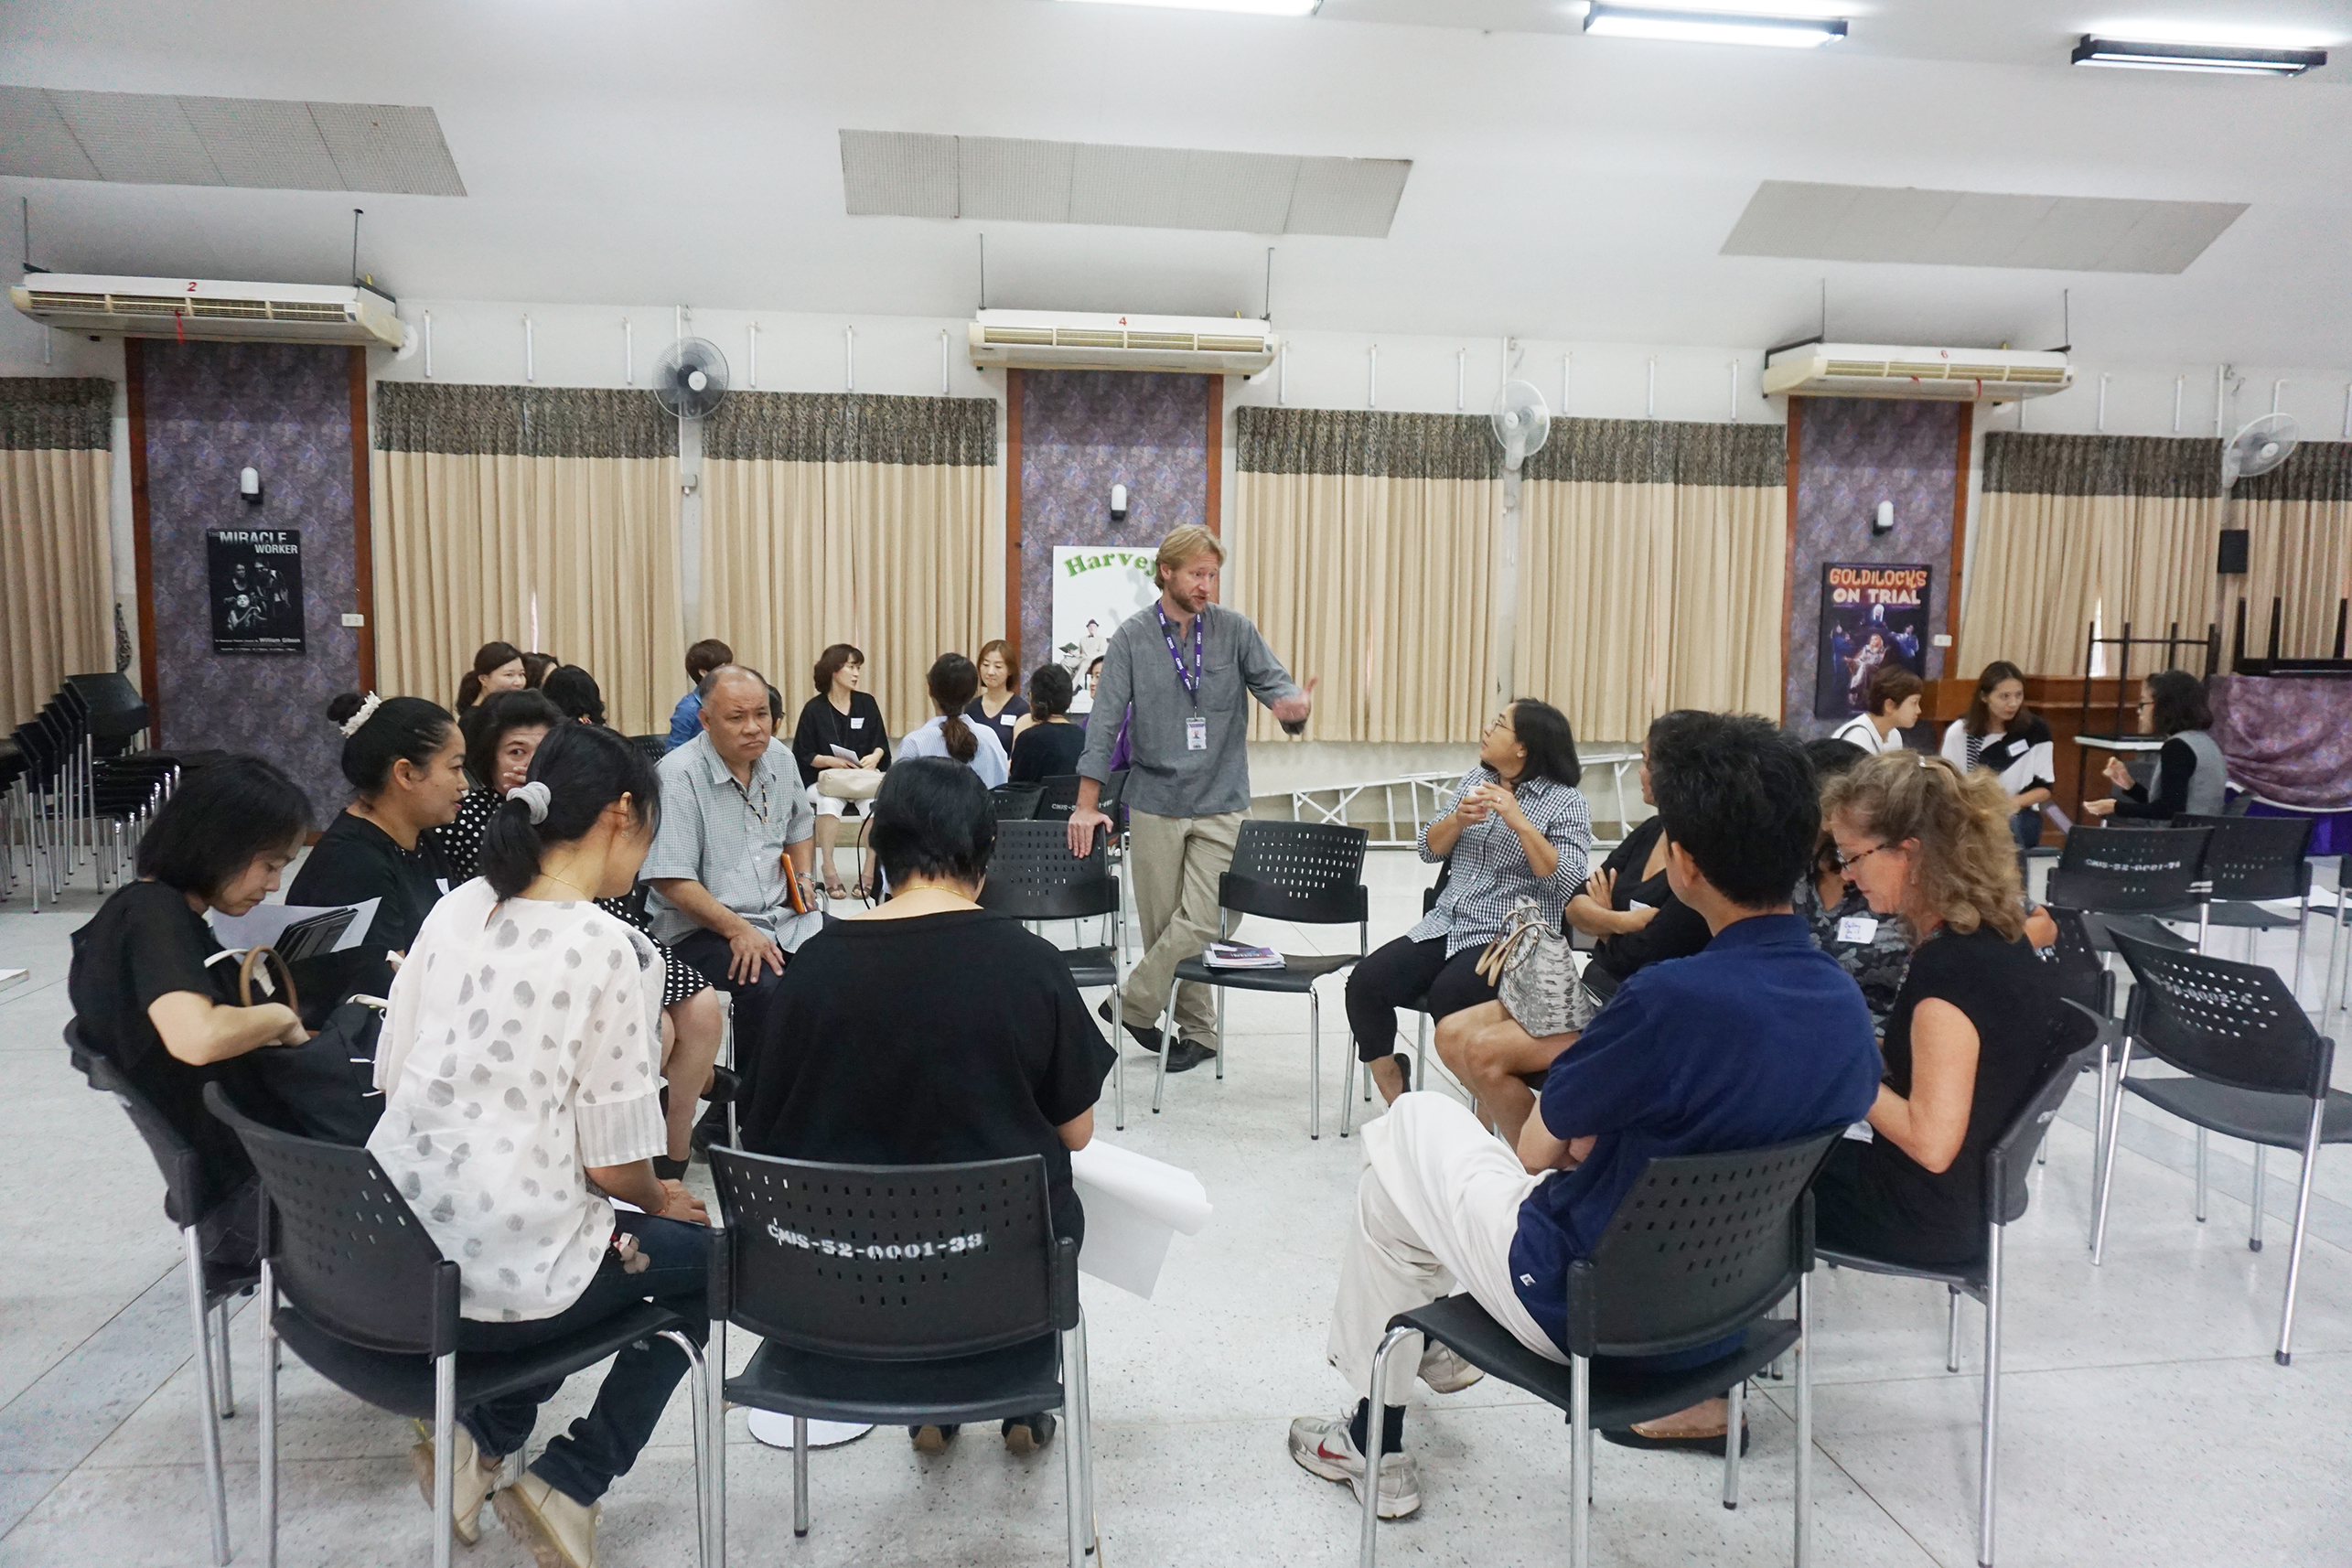
\includegraphics[width=\textwidth]{chapter4_a3.JPG}}


\minor{Additional Structures for Collaboration}

In addition, monthly Team Meeting Time and \href{https://docs.google.com/document/d/1tSEBD59kwf83Z0-m1Q4hzNrVwaJMHdracrghwqoSdW0/edit?ts=589d238c}{Early Release Professional Developments Days} are held for all teachers to collaborate, review student work, and plan instructional practices to improve student achievement. In addition, the faculty regularly reviews the definition of global citizenship during their professional development meetings and brainstorm ways for our students to practice being responsible, proactive members of the global community (e.g. \href{https://docs.google.com/a/cmis.ac.th/document/d/1fJmuufIbXlGt7DGAuQ3OBW00VdOY_1QgqLzgEpmxdKQ/edit?usp=sharing}{Cultural Heritage Flag Communication Group Activity}).

\href{https://docs.google.com/document/d/1eDtOzhe_JnpVQmEIoF-IO0ejVrDalm8s0i6PaiDl9hs/edit}{Instructional Rounds process}: see Curriculum, Instruction, and Assessment Chapter for more information. 

The K-12 Student Success Team has implemented Response to Intervention (RTI) model as a way of supporting all students and teachers through the use of positive (academic and behavioral) interventions. See the \href{https://docs.google.com/document/d/16bGCvdQuhHquFdigvip3H5YgfubNVMStl7UpOfCRcFk/edit}{Behavior Management Plan} for evidence. 

The \href{https://docs.google.com/a/cmis.ac.th/document/d/1iW_tWIwRlWU2p0oIOvd3usDsxj9qYDt_2ROwNPBTHSc/edit?usp=sharing}{Teacher Leadership Team} was established during the 2015-16 school year. This team of ten teachers was created to increase staff leadership roles and promote a shared responsibility and accountability to support student learning in a global environment. The team meets 3-4 times a semester with the administrative team to collaborate on ways to support PK-12 teachers with: instructional best practices, curriculum planning, assessment design, and data analysis. Meetings also review specific leadership skills such as facilitating meetings, creating a plan of action, and monitoring team progress.

In all divisions, the \href{https://docs.google.com/document/d/15_5X5QtixmWVheEUBVO9N1aislsLDm_ZW4-4g4YQ7F4/edit?ts=589d25d9}{teacher evaluation process}, regular classroom walkthroughs and informal and formal observations have all been modified and increased to further ensure collaboration and accountability for enhanced student learning.

\minor{So what}

Though the CMIS Leadership has developed multiple  initiatives for staff to increase shared responsibility, accountability, and collaboration opportunities.  In the future, CMIS will be including a more frequent focus on looking at student evidence to help in evaluating the effectiveness of these current initiatives. 
\end{findings}

\subsubsection{Evaluation of Existing Processes}

\indicator{The school leadership regularly reviews the existing processes to determine the degree to which actions of the leadership and staff focus on successful student learning and global citizenship.}

\prompt{To what extent does the school leadership regularly review the existing processes to determine the degree to which actions of the leadership and staff focus on successful student learning? Evaluate the effectiveness of the school leadership and staff to work collectively as a learning community in order to promote the desired global competencies.}

\begin{findings}
CMIS leadership regularly review existing processes to determine the degree to which actions of the leadership and staff focus on successful student learning and global citizenship.

In 2014 all teachers were trained and have since participated in the year long \href{https://drive.google.com/a/cmis.ac.th/file/d/0B71_pYxcTLo-OExlV0Y5UVFBNVU/view?usp=sharing}{Datawise Process}. Data Wise a school improvement process that organizes and brings coherence to the work of improvement. It is a specific process that facilitates intentional thinking and utilizing a more disciplined way of looking at student data as a collaborative group. Datawise helps all educators in all positions to learn how to analyze data in a manner that contributes to improved instruction and increased student learning. \href{https://docs.google.com/document/d/1TmnCp5qZiZAUMnUmaU32PBn2UGvCMVtFO8r5OsxwNo4/edit}{CMIS 2016-17 Datawise Plan}

Since 2014 all staff  have incorporated the \href{https://docs.google.com/a/cmis.ac.th/document/d/1IFIRIT2wAu1GF2yZ5FSSOdFB3yBKxzx_eCZhdFtroC0/edit?usp=sharing}{Datawise} agenda template when collaborating with colleagues. This template includes reviewing the norms of engagement, that the objective is aligned to increasing student learning, and that there is an assessment of how useful the meeting was in accomplishing the goal.

During the 2015-16 school year CMIS organized \href{https://drive.google.com/a/cmis.ac.th/file/d/0ByVFfrm0zfolbHNvSWhVWmJYU3M/view?usp=sharing}{Teacher Table Talk} sessions during early release days for staff to capture insights and suggestions about successful ways to increase student learning and promote global citizenship.

\minor{\href{https://drive.google.com/drive/folders/0ByVFfrm0zfolLTd2WjVNX0pWZU0?usp=sharing}{Instructional Rounds}}

Instructional Rounds were implemented at CMIS in 2015. They are structured observations between teachers and during the instructional round period, a great deal of data is collected which focus on teacher deliberative practice and student achievement. See sections entitled: Congruence and Collaborative Work for more information on instructional rounds. 

\minor{So what}

A great deal of evaluation of the processes to determine student achievement have taken place over the past three years. For example, the initial review of the teacher evaluation instrument and process was found not to be aligned with current research or student achievement. CMIS Leadership and volunteer staff collaborated in piloting a more inclusive model prior to training all new staff the following year. This allowed CMIS to modify and adjust the process and ensure that student learning was the focus. 

The \href{https://drive.google.com/a/cmis.ac.th/file/d/0B71_pYxcTLo-OExlV0Y5UVFBNVU/view?usp=sharing}{Datawise process} has enabled CMIS Leadership and Staff to identify authentic areas for instructional improvement. For example, during the 2015-2016 school year, lack of consistent assessments among divisions was identified as a need and has been the focus for this year’s \href{https://docs.google.com/a/cmis.ac.th/document/d/1ioGkUkxTr5hRC_Vn4TDy7FcKHwcaWzBYNEeIConfXA4/edit?usp=sharing}{Datawise Department Action Plan}. CMIS should continue to implement the Datawise process with fidelity in order to meaningfully identify further areas for future improvement in student achievement.
\end{findings}
